Online anomaly detection (OAD) is the task of identifying deviations from the normal behavior in a streaming fashion, where samples arrive sequentially, and decisions must be made before the next sample is received. This task plays a fundamental role in various practical applications within cyber and cyber-physical systems, including maintenance \cite{khan2020industrial}, monitoring \cite{hill2010anomaly}, and security \cite{mirsky2018kitsune, lazarevic2003comparative}. In modern environments, the sheer volume and velocity of data make it often impractical to have comprehensive labels for all anomalous samples \cite{siffer2017anomaly, schmidl2022anomaly, ren2019time, audibert2020usad}.

In deployment, typical AD algorithms assign a real-valued anomaly score to each sample, where a higher score indicates a greater degree of anomaly \cite{chandola2009anomaly}. The OAD algorithm first scores each sample and then calibrates a threshold to make the binary decision of whether the given sample is anomalous or not. The choice of this threshold is critical due to its significant downstream impact. In security systems, for example, failing to detect a genuine anomaly or security event can have catastrophic consequences \cite{203674}. Conversely, false positives incur costs, as each detection necessitates investigation by a security operator, potentially leading to `alert fatigue' \cite{202751, lin2018collaborative, he2023cloudshield}.

Given the risk of incorrect decisions, a common methodology to set the threshold is by \emph{abstaining} from decisions for an initial `cold-start' number of samples on the  stream \cite{10.14778/2850583.2850593, katz2023cold}. At the end of the cold-start period, a threshold is chosen for future decision making, either by algorithm or by an expert based on the online scores during the cold-start, as well as any offline data that is available \cite{ren2019time, bhatia2021mstream,huang2022semi, li2021fluxev}. 
This approach has two drawbacks. 
Firstly, using a fixed cold-start duration across all streams independent of stream statistics is sub-optimal and can lead to much more abstains than necessary. Secondly, a static threshold is prone to performance loss when the data stream undergoes distribution shift - a common occurrence in many AD systems \cite{279982,gama2014survey}. Although adapting anomaly scoring to distribution drifts have been studied \cite{ma2018robust,bhatia2022memstream, sankararaman2022fitness}, limited advances have occurred in adapting the threshold dynamically.
%We frame the threshold selection as online quantile estimation and provide guarantees on number of false positives and false negatives that hold even under distribution shifts and provably improve in the presence of offline data. 
%
%scores gathered thus far  (cf. Fig \ref{fig:static_cold_start}). If appropriate, offline data is used along side the online scores during cold-start to minimize risks of incorrect decisions \cite{ren2019time, bhatia2021mstream,huang2022semi, li2021fluxev}. 


%\subsection{Threshold selection as quantile estimation}

We formulate adaptive threshold selection as online quantile estimation by defining anomalies as tail quantile of anomaly scores \cite{steinwart2005classification, cadre2013estimation, gan2017scalable, siffer2017anomaly}. Formally, we model that each time $t \in \mathbb{N}$, the anomaly score $S_t \in \mathbb{R}$ is independently sampled from distribution $f_t$. This score $S_t$ is an {anomaly} if it exceeds the $p$th quantile of the distribution $f_t$. We assume the quantile level $p \in (0,1)$ is known, while the distribution $f_t$ as unknown to the algorithm. 
Knowledge of $p$ arises either from a constraint on the rate of anomalies that can be investigated without succumbing to alert fatigue \cite{hassan2019nodoze, ho2021hopper}, or from domain knowledge \cite{perini2023unsupervised}. 

Performance of threshold selection is measured by false positives (FP), benign samples marked as anomalous, false negatives (FN), anomalous sample mark as benign, and number of samples abstained from making a decision on. Since AD outputs are typically used to make consequential decisions, e.g. engaging human operators to triage alerts, OAD systems must achieve low number of FPs and FNs, by possibly trading-off with abstains \cite{ho2017detecting}. Further, these systems need to be adaptive to distribution shifts and be designed without requiring distributional assumptions (cf. \emph{Research challenges} $5$-$7$ of \cite{sadik2014research}).

 \subsection{Desiderata of OAD threshold selection systems}
 \label{sec:desiderata}

% AD Threshold systems marks each sample as either anomalous, non-anomalous or abstains from decision making \cite{chandola2009anomaly}. Performance is measured by false positives (FP), benign samples marked as anomalous, and false negatives (FN), anomalous sample mark as benign, in addition to number of samples abstained on. Typically, since AD outputs are used to make consequential decisions, e.g. engaging human operators to triage alerts, OAD systems must have low number of FPs and FNs achieved at the cost of abstains \cite{ho2017detecting}. Further, these systems need to be adaptive to distribution shifts and be designed without requiring distributional assumptions (cf. \emph{Research challenges} $5$-$7$ of \cite{sadik2014research} and references therein). In summary, the following set of statistical requirements are desired.

 %the following set of statistical requirements desired for online threshold selection. \cite{sadik2014research}.
 
In summary, the following set of statistical requirements is desired for online threshold selection.
 
    \emph{\textbf{(i) High accuracy:}} Constant number of mistakes\footnote{Throughout, we denote the mistakes as sum of FP and FN.} independent of the stream length on an i.i.d. data-stream.

      \vspace{-1mm}
     \emph{\textbf{(ii) Low abstention:}} Abstain on a vanishing fraction of samples on an i.i.d. stream, i.e. small cold-start period. 

     \vspace{-1mm}
    \emph{\textbf{(iii) Adaptive to distribution changes:}} On a non-stationary stream, number of mistakes and abstains only increase compared to the stationary setting by a constant factor that is independent of the stream length, but only proportional to the number and magnitude of distribution changes. 
    
    \vspace{-1mm}
       \emph{\textbf{(iv) Learn from offline dataset:}} When unlabeled offline datasets are available, abstain rate is a constant independent of stream length, as long as the online distribution matches one of the offline distribution. In the worst-case of arbitrary offline dataset distribution, performance degradation compared to no offline dataset must be bounded independent of stream length and size of the dataset.

       \vspace{-1mm}

       \emph{\textbf{(v) Distribution and parameter free:}} The algorithm does not require any knowledge of the distributions or assumptions such as sub-gaussian tails or parameterized distribution family, and nevertheless must guarantee all of above.
     %The algorithm however does not know apriori if the online stream and offline dataset are from the same distribution.
% \begin{enumerate}[itemsep=0pt,topsep=-2pt, labelindent=-1pt,labelwidth=!]
%     \item \textbf{High accuracy:} Constant, independent of the stream length, number of mistakes\footnote{Throughout, we denote the mistakes as sum of FP and FN.}, on an i.i.d. data-stream.
%     \item \textbf{Low abstention:} Abstain on a vanishing fraction of samples on an i.i.d. stream, i.e., small cold-start period. 
%     \item \textbf{Adaptive to distribution shifts:} On a non-stationary stream, the FPs, FNs and abstains only increase compared to the stationary setting by a constant factor that is independent of the stream length, but only proportional to the number and magnitude of distribution changes. The algorithm however cannot know apriori the number of changes on the stream.
%     \item \textbf{{\color{black} Learn from offline data:}} If there is access to multiple unlabeled offline datasets, then the fraction of abstains is a constant independent of stream length, whenever the online distribution matches one of the offline distribution. However, if none of the offline distributions matches the online stream, the performance must be comparable to the setting without offline data. %The algorithm however does not know apriori if the online stream and offline dataset are from the same distribution.
%     \item \textbf{Distribution and parameter free:} The algorithm does not require any knowledge of the distributions or assumptions such as sub-gaussian tails or the distribution family being parameterized, nevertheless must guarantee all of the aforementioned performance.
% \end{enumerate}

%Crucially, we want the above desiderata to be satisfied without any assumptions on the distribution such as tails or parametric form. 




%The online version of the unsupervised AD problem is one where samples are presented to the AD algorithm one at a time in a streaming fashion. At each time step, the AD algorithm outputs an anomaly score based on the samples seen thus far. As the problem is unsupervised, the ground-truth label of the sample is not available to the AD algorithm before making its next set of predictions. This unsupervised, OAD is a common abstraction for many problems in cloud-computing, performance monitoring and network intrusion detection systems .

%Typical performance measures of anomaly detection algorithms are AUC (Area under the curve) of the ROC (Receiver operating curve). This measure is computed by comparing the anomaly scores output by the AD algorithm and the ground-truth binary labels by sweeping over all possible choice of anomaly thresholds. However, 

% \paragraph{Anomaly thresholding.}  Most modern AD algorithms outputs an anomaly score for a given sample and are evaluated using threshold-agnostic metrics such as AUCROC. The choice of how to choose a threshold is often left unstudied and unreported. This is especially surprising since in practice, tuning thresholds is an important problem and critical to the performance of any AD system \cite{chandola2009anomaly, hundman2018detecting} 


\subsection{Main result and technical contributions}

{Algorithm \ref{alg:five} is distribution and parameter free and is the \emph{first algorithm to satisfy all the aforementioned desiderata.}}  Algorithm \ref{alg:five} does not require knowledge on the locations or number of distribution shifts nor on the online stream or the offline datasets' distributions. Nevertheless, under mild technical assumptions, the guarantees in Theorem \ref{thm:core_theorem} show that the performance adapts to the problem complexity.
%, if any stationary segment of the online stream matches any of the offline datasets' distirbution, the number of abstains and mistakes are small. On the other hand if a stationary segment in the online distribution is arbitrary and does not match any offline datasets' distribution, then the performance on this segment is comparable to one in which no offline data is present.
%However, the algorithm does not need as input any prior information, but rather its performance adapts to the complexity of the online data stream. 
%In particular, FP, FN and abstain are lower when there is fewer distribution shifts and/or offline datasets have the same distribution as the online stream, with the bounds naturally identifying the problem complexity parameter. 
%\subsection{Technical Contributions}
Concretely, our contributions are as follows.

{\color{black} \textbf{1. High accuracy requires abstention.} We prove that any  scheme that does not abstain,  cannot achieve constant FPs and FNs, even for a stationary stream. The proof follows by constructing a hard instance and a reduction from decision making to hypothesis testing on that instance. }

{\color{black} \textbf{2. Algorithm using confidence sequences (CS) to adapt threshold to distribution changes.} 
%  Threshold using confidence sequence (CS) to be adaptive to changes in distribution.
%We connect OAD and threshold selection with confidence sequences (CS). 
%We use  CS to make decisions to yield high-accuracy and a data-dependent abstain. 
A sample $S_t$ is deemed as an anomaly by our algorithm (Algo. \ref{alg:five}) if it exceeds the upper confidence of the $p$th quantile,  is benign if it is smaller than the lower confidence, and is abstained from otherwise (Fig. \ref{fig:motivation_alg_1}). The crux of our algorithm is in choosing the \emph{relevant online and offline samples} to construct the CS. Online distribution shifts are detected by constructing CS on different sub-sequences and testing if they have a non-empty intersection. Theorem \ref{the:iid} shows that on an i.i.d. stream of length $T$, no mistakes  and at-most $\mathcal{O}(\sqrt{T})$ abstains occur with high probability. 
%3. \textbf{Confidence sequences can provably be adaptive to distribution shifts.} 
Theorem \ref{thm:online_shift} shows that when there are distribution shifts, our algorithm incur total additional mistakes \emph{independent} of $T$, without requiring any knowledge of the data distributions or change-points.
%our algorithm, without requiring any knowledge of the distributions or change-points, incurs an additional factor \emph{independent} of $T$ mistakes and abstains compared to the stationary stream.

% The CS for the $p$th quantile is a sequence of random intervals $([l_t, u_t])_{t \geq 1}$ such that for all $t \geq 1$, {\em(i)} $l_t \leq u_t$ almost-surely are measurable functions of $S_1, \cdots, S_t$, and {\em(ii)} with high probability, the intersection of all intervals contains the true quantile \cite{howard2022sequential}. 
% %The existence and construction of CS  are shown in \cite{howard2022sequential}. 
% Algorithm \ref{alg:five} declares $S_t$ anomalous if $S_t > u_t$, benign if $S_t < l_t$ and abstain otherwise (Figure \ref{fig:motivation_alg_1}). Distribution shifts are detected in Algorithm \ref{alg:five} by constructing CS on different sub-sequences and testing if they have a non-empty intersection.  Theorem \ref{the:iid} shows that on an i.i.d. stream of length $T$, no mistakes  and at-most $\mathcal{O}(\sqrt{T})$ abstains occur with high probability. 
% %3. \textbf{Confidence sequences can provably be adaptive to distribution shifts.} 
% Proposition \ref{prop:dist_changes} shows that on a non-stationary stream, the mistakes and abstains only increase by a constant factor depending on the magnitude of distribution shifts, while Algorithm \ref{alg:five} does not require any knowledge of the distributions.

\textbf{3. Relevant offline dataset improves online performance, while irrelevant offline dataset has bounded degradation.} Theorem \ref{thm:core_theorem} proves that when offline data matching the distributions of the online stream are available, they improve abstain rate without loss of accuracy. In the \emph{worst-case} when the offline dataset's distributions are arbitrary, the performance degradation compared to the case when the algorithm ignores offline dataset is \emph{bounded independent of stream length or offline dataset size}. Algorithm \ref{alg:five} does not a priori know if the offline dataset is useful or not, but yields improved guarantees whenever the offline dataset is useful. The technical novelty is to rely on an offline dataset \emph{only if a CS constructed on offline dataset} intersects with the online CS. This is the first algorithm for online thresholding showing improved  performance in the presence of useful offline data, while guaranteeing worst-case bounds if the offline data is arbitrary. 
%Previous methods for this only relied on heuristics \cite{audibert2020usad, bhatia2022memstream, huang2022semi} 

%4. \textbf{Empirical.} Superior performance in terms of FP, FN and abstains compared to baselines and heuristics, both on real and synthetic data.

}

%\vspace{-0.5em}
% \paragraph{1 and 2. High Accuracy and Low Abstention : Confidence-sequences as adaptive cold-start.} Our primary contribution is to make rigorous the connection between OAD and threshold selection with confidence sequences (CS). The CS for the $p$th quantile is a sequence of random intervals $([l_t, u_t])_{t \geq 1}$ such that for all $t \geq 1$, {\em(i)} $l_t \leq u_t$ almost-surely are measurable functions of $S_1, \cdots, S_t$, and {\em(ii)} with high probability, the intersection of all intervals contains the true quantile \cite{howard2022sequential}. 
% %The existence and construction of CS  are shown in \cite{howard2022sequential}. 
% Given a CS, Algorithm \ref{alg:five}  makes decisions on an i.i.d. sequence by declaring a sample $S_t$ anomalous if $S_t > u_t$, benign if $S_t < l_t$ and abstain if $l_t \leq S_t \leq u_t$ (Figure \ref{fig:motivation_alg_1}). We show in Theorem \ref{the:iid} that our algorithm guarantees that there are $0$ FP and FN and at-most order $\sqrt{T}$  abstains over $T$ samples, with high probability. 

% \vspace{-0.5em}
% \paragraph{3. Adaptivity to distribution shifts.} We use the CS to also detect distribution shifts, by deeming a shift to have occurred if the CS on two sub-sequences of points $S_1, \cdots, S_t$ are non-intersecting \cite{shekhar2023sequential, sankararaman2023online}. Our result in Proposition \ref{prop:dist_changes} shows, that the number of FPs and FNs only scale with the number of distribution shifts, even when the algorithm has no knowledge of the number and location of distribution changes.

%\vspace{-0.5em}
%\paragraph{4. Efficiency: Provably improving online performance in the presence of offline datasets.} 
%Our most general result is in Algorithm \ref{alg:five} whose performance guarantee is stated in Theorem \ref{thm:core_theorem}. This general result assumes that at each time, in addition to all the samples on the stream observed thus far, the AD system also has access to a \emph{offline dataset}. 
% In Theorem \ref{thm:core_theorem}, we prove that when an offline dataset is available, the following two desiderata can be achieved \emph{simultaneously}. If the online stream has the same distribution as one the offline datasets, then improved performance in terms of FP, FN and abstain are observed as opposed to not using the offline data, and if the online stream's distribution does not match any offline dataset, then the performance is comparable to the performance in the absence of any offline dataset. In particular, Theorem \ref{thm:core_theorem} proves that desiderata $4$ from Section \ref{sec:desiderata} is achieved by Algorithm \ref{alg:five}. The algorithmic novelty is to rely on an offline dataset only if a CS constructed on offline dataset intersects with the online CS. This is the first provable strategy of improved thresholding performance in the presence of offline data, while methods relied on heuristics \cite{audibert2020usad, bhatia2022memstream, huang2022semi} 

%that using an offline dataset is algorithmicaly similar to detecting a change-point, namely the online stream matches the offline if the CS from the offline and online stream overlap. 

%This setting is also of practical importance as it is a common occurrence in AD systems in several cloud-computing and IoT settings \cite{sauvanaud2018anomaly,islam2021anomaly, 235002}. However, our results are the first provable algorithm with guarantees on FP, FN and the number of abstains.  \abishek {Flex on how theory is SOTA.}

\begin{figure}
\centering
\begin{subfigure}{.48\columnwidth}
  \centering
  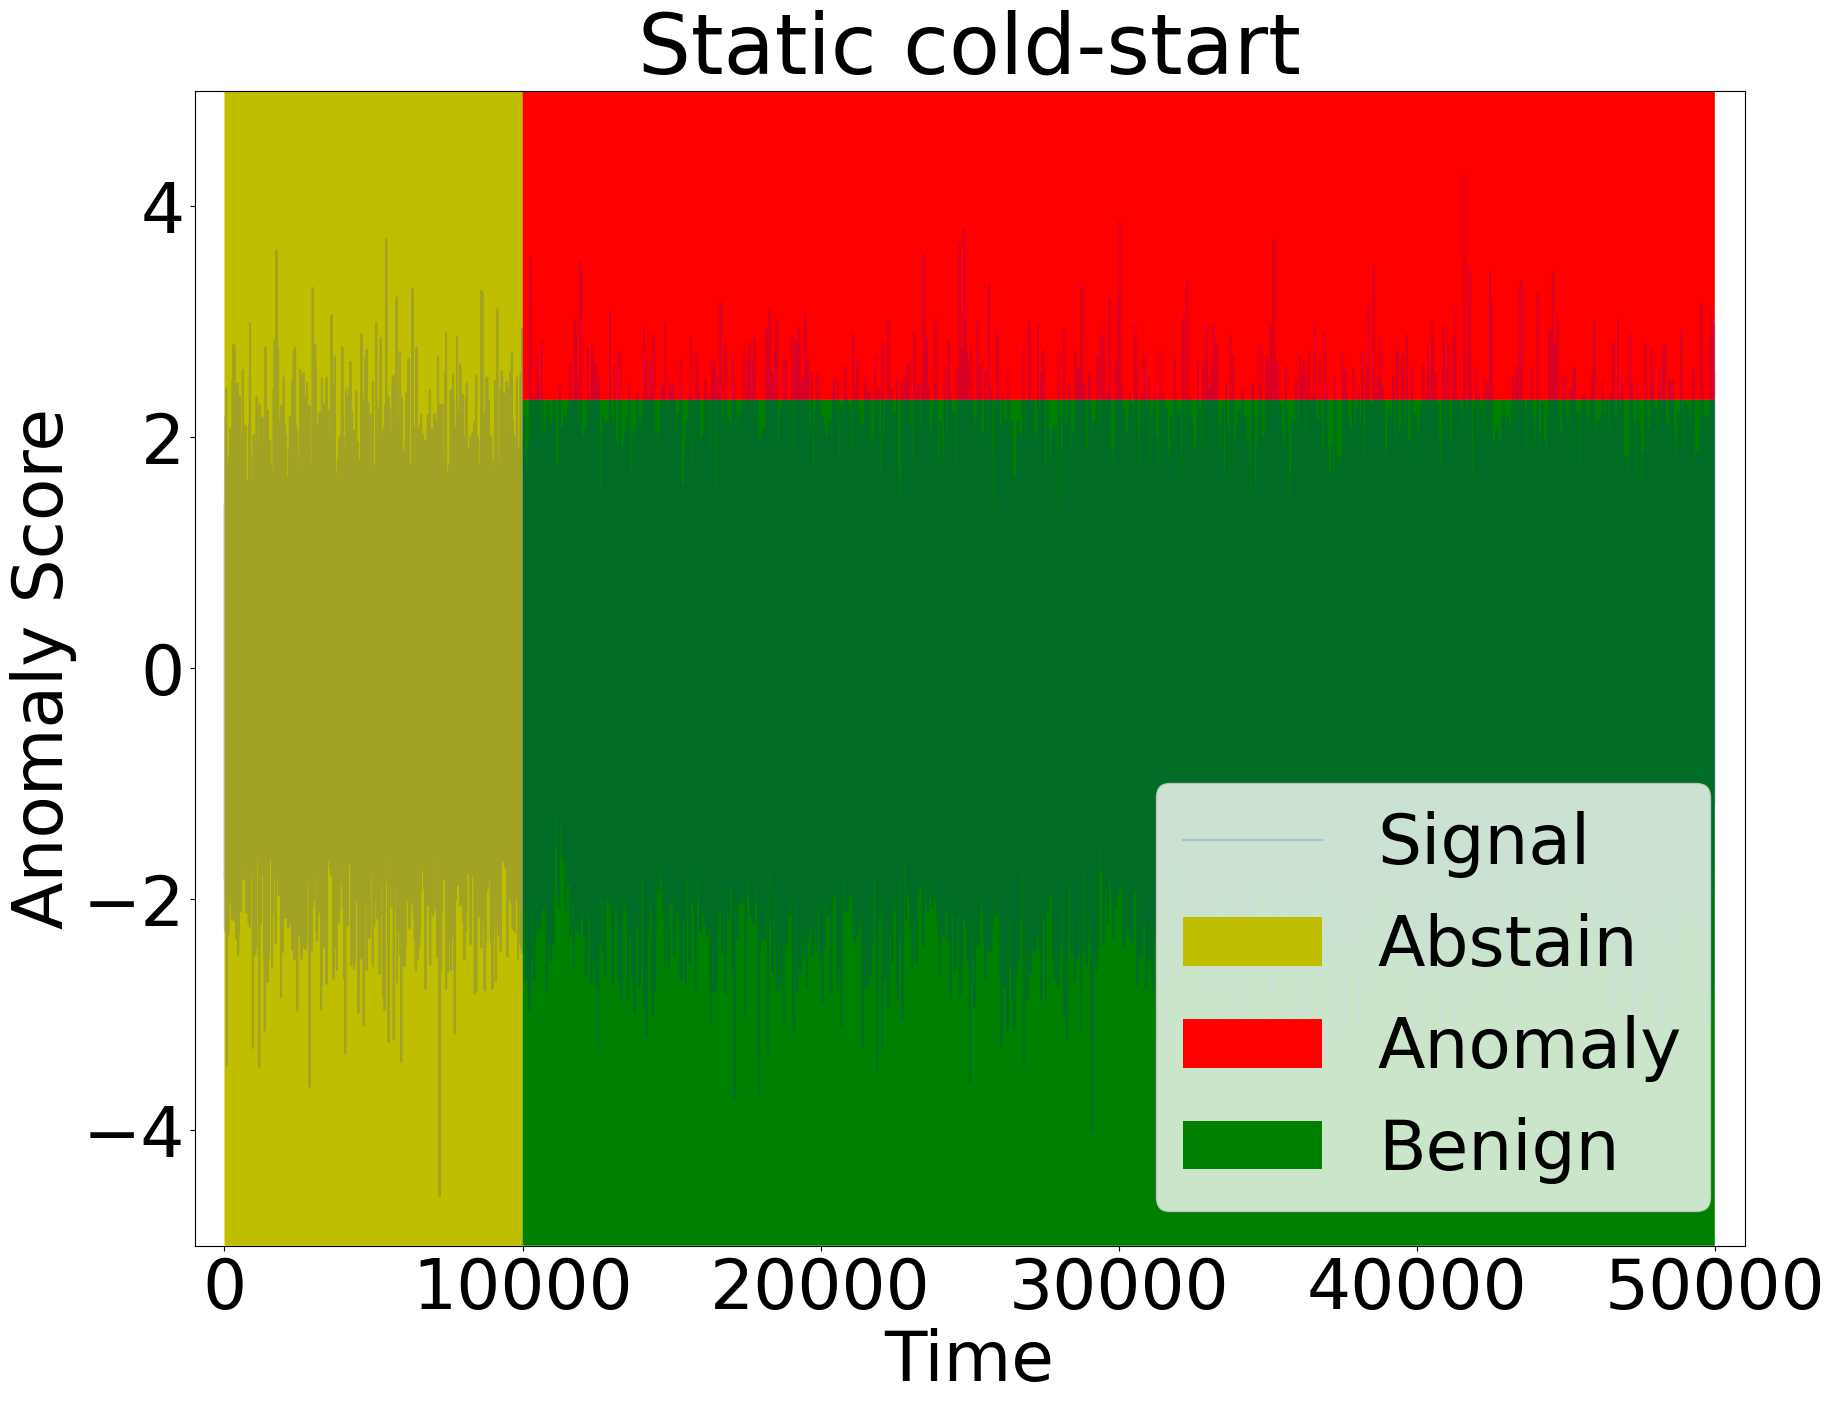
\includegraphics[width=\linewidth]{anomaly/figs/static_cold_start.png}
  %\caption{Anomaly threshold set using a fixed cold-start period}
  \caption{}
  \label{fig:static_cold_start}
\end{subfigure}%
\begin{subfigure}{.48\columnwidth}
  \centering
  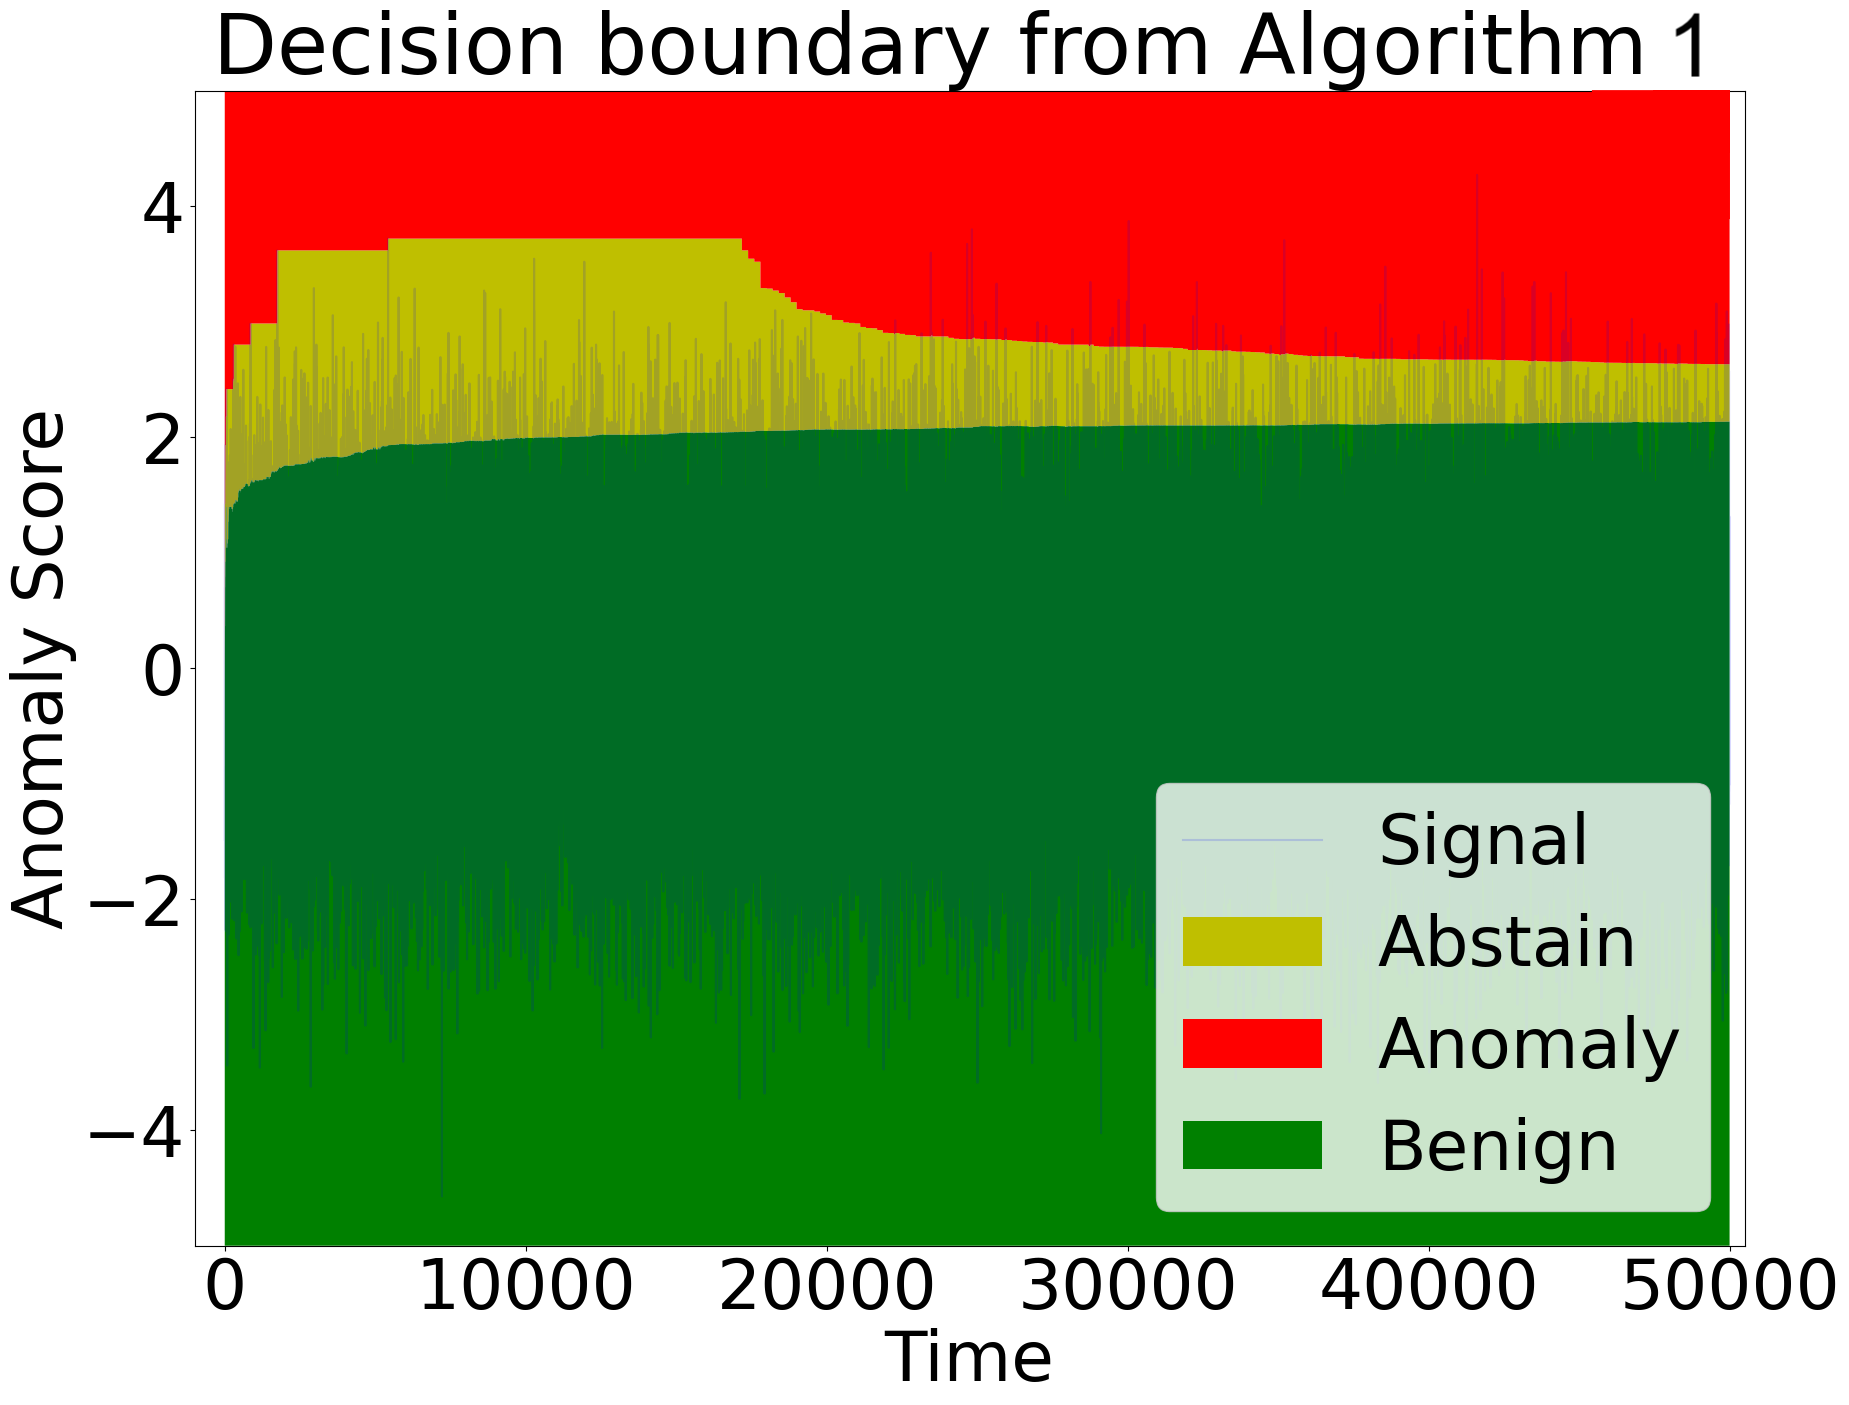
\includegraphics[width=\linewidth]{anomaly/figs/algo1_example.png}
  %\caption{A subfigure}
  \caption{}
  \label{fig:sub2}
\end{subfigure}
\vspace{-0.5em}
\caption{Fig $(a)$ is the heuristic of a fixed cold-start where all samples are abstained from and a static threshold for all future samples. Fig $(b)$ is the decision boundary from Algorithm \ref{alg:one} using an adaptive cold-start.}
\label{fig:motivation_alg_1}
\vspace{-1.5em}
\end{figure}





% AD algorithms abstain by relying on an initial cold-start period. At the end of the cold-start period, the AD system will use the samples seen and any offline information to choose an appropriate threshold \cite{audibert2020usad, chandola2009anomaly}. 




% We introduce abstaining as a possible output of an AD algorithm, in addition to the canonically binary output of anomaly and benign data. The abstain option can be viewed as a data-adaptive, more flexible framework of the cold start period that is commonly used to tune the anomaly threshold. In this paper we include abstaining into the regret metric, to analyze its trade off with making false positive and false negative errors.  

% \paragraph{Leveraging offline datasets to improve online performance, provably}


% \paragraph{Finite-sample, distribution free guarantees on performance}

% \paragraph{Contributions} We are the first work to systematically study the problem of unsupervised anomaly thresholding. We propose algorithms in various settings, and provide a principled framework to analyze their performance. Our contributions are: 

% \begin{enumerate}
% \item {\color{red} Our method provides a statistical framework to tune anomaly thresholds in an online fashion. Our methodology picks a `cold-start' period that is data dependent. Anomalies that are harder to distinguish have a larger cold-start than those that are easier to distinguish.
% Thus, our methodology gives a principled generalization of the common heuristic of having a fixed cold-start period. }
%     %\item Our algorithm improves upon the manually tuned anomaly thresholding with cold-start period commonly used in practice, and provide an algorithm where abstaining is adaptive and data-dependent.
%     \item We prove guarantees on false positive and false negative rates, and number of abstains. {\color{red} 1-2 sentences on the novelty/difficulty}
%     \item We prove that our algorithms and guarantees are adaptive to online distribution shifts. {\color{red}1-2 sentences on how we connect the detection delay with the mistake bounds.}
%     \item Our algorithms leverages offline data to improve online performance with best of both worlds results: it significantly lowers number of abstains when offline data is available, and reduces to online algorithm when it is not. {\color{red} Our algorithm is the first to rigorously show the best of both worlds for online threshold selection?}
% \end{enumerate}

%Our work shows how to tune parameters to achieve. We also show conditions when presence of offline data can improve online performance.....



% \section{Related Work}%\vspace{-0.5em}
% \paragraph{Dynamic thresholding for AD.} AD is an extensively researched topic, where a common paradigm is to first model data likelihood and then use a threshold to decide if a data point is normal or anomalous. This threshold is typically determined by an expert or empirically, see surveys \cite{luo2021deep, schmidl2022anomaly}. Dynamic and automatic methods makes AD algorithms more practical in real-world deployment \cite{ali2013automated, hundman2018detecting}, and are necessary where the data distribution can shift \cite{siffer2017anomaly}. 

% %\cite{siffer2017anomaly, , hundman2018detecting}
% %This work instead focuses on providing a principled analysis of the thresholding step that follows. Traditionally, and are chosen by heuristics . Works closer to us are thresholding algorithms for univariate online streams .
% %\vspace{-0.5em}
% \paragraph{Confidence Sequences.} We use theoretical results and tools of confidence sequences (CS) for our analysis \cite{ramdas2022game}. \cite{maharaj2023anytime, howard2022sequential} derived the CS algorithm for estimating quantiles online with any-time guarantees, and \cite{shekhar2023sequential} leverages CS's consistency property for detecting distribution shifts. These tools allows us to bound the false positive and negative rates of our algorithm.

% {\color{red} \paragraph{Threshold learning systems.}
% Threshold scores to make the binary decision have been studied in active learning to make the decision of  seeking labels from experts \cite{balcan2007margin, zhang2016online,vishwakarma2023promises}. However, active learning does not have a concept of mistakes and is thus different from ours. 

% }